\documentclass[notitlepage]{ctexrep}
\usepackage{amsmath,amsfonts,amsthm,amssymb}
\usepackage{authblk}
\usepackage[T1]{fontenc}
\usepackage{graphicx}
% \usepackage[utf8]{inputenc}
\usepackage{newunicodechar}
\usepackage[framemethod=tikz]{mdframed}
\usepackage{natbib}
\usepackage{subcaption}
\usepackage{tikz}
\usepackage{xcolor}
\usepackage{epigraph}
\usepackage{float}


%设置超链接
\usepackage[colorlinks,linkcolor=blue,
citecolor=red]{hyperref}


\definecolor{blue}{RGB}{38,139,210}
\definecolor{cyan}{RGB}{42,161,152}
\definecolor{violet}{RGB}{108,113,196}
\definecolor{red}{RGB}{220,50,47}
\definecolor{base01}{RGB}{88,110,117}
\definecolor{base02}{RGB}{7,54,66}
\definecolor{base03}{RGB}{0,43,54}

\usetikzlibrary{calc,shapes,positioning}

\newcommand{\todo}[1]{\textcolor{red}{TODO: #1}}

\newtheorem{relationship}{关系}
\providecommand*{\relationshipautorefname}{关系}
\surroundwithmdframed[
    topline=false,
    bottomline=false,
    middlelinewidth=0.5pt,
    linecolor=base01,
    roundcorner=5pt,
    innertopmargin=0pt,
    leftmargin=15pt,
    rightmargin=15pt,
    nobreak=true,
]{relationship}

\setcounter{MaxMatrixCols}{16}

\let\originalepigraph\epigraph
\renewcommand\epigraph[2]{\originalepigraph{\textit{#1}}{\textsc{#2}}}

% Use arabic numbers for thanks
\makeatletter
\let\@fnsymbol\@arabic
\makeatother

\title{深度学习卷积运算指南}
\author[$\bigstar$]{Vincent Dumoulin\thanks{dumouliv@iro.umontreal.ca}}
\author[$\bigstar\dagger$]{Francesco Visin\thanks{francesco.visin@polimi.it}}
\affil[$\bigstar$]{MILA, Universit\'{e} de Montr\'{e}al}
\affil[$\dagger$]{AIRLab, Politecnico di Milano}
\date{2018.1.12}

\begin{document}

\maketitle
\thispagestyle{empty}
\clearpage

\setlength{\epigraphwidth}{0.4\textwidth}
\epigraph{All models are wrong, but some are useful.}{George E. P. Box}
\clearpage

\renewcommand{\abstractname}{Acknowledgements}
\begin{abstract}
    The authors of this guide would like to thank David Warde-Farley, Guillaume
    Alain and Caglar Gulcehre for their valuable feedback. We are likewise
    grateful to all those who helped improve this tutorial with helpful
    comments, constructive criticisms and code contributions. Keep them coming!

    Special thanks to Ethan Schoonover, creator of the Solarized color
    scheme,\footnote{\url{http://ethanschoonover.com/solarized}} whose colors
    were used for the figures.
\end{abstract}

\renewcommand{\abstractname}{Feedback}
\begin{abstract}
    Your feedback is welcomed! We did our best to be as precise, informative and
    up to the point as possible, but should there be anything you feel might be
    an error or could be rephrased to be more precise or comprehensible, please
    don't refrain from contacting us. Likewise, drop us a line if you think
    there is something that might fit this technical report and you would like
    us to discuss -- we will make our best effort to update this document.
\end{abstract}

\renewcommand{\abstractname}{Source code and animations}
\begin{abstract}
    The code used to generate this guide along with its figures is available on
    GitHub.\footnote{\url{https://github.com/vdumoulin/conv_arithmetic}} There
    the reader can also find an animated version of the figures.
\end{abstract}

\tableofcontents

\chapter{引言}

深度卷积神经网络 (CNNs) 一直是深度学习取得巨大进步的核心. 尽管卷积神经网络在九十年代就被用来解决字符识别任务\citep{le1997reading},它们当前的广泛应用是由于最近的工作,当时一个深层CNN被用来打败最先进的ImageNet图像分类挑战\citep{krizhevsky2012imagenet}.

因此卷积神经网络为机器学习的专业人士构建了一个非常有用的工具. 然而,第一次学习使用卷积神经网络通常是一种``可怕''的经历. 一个卷积层的输出形状受它的输入形状及卷积核的形状、零填充和步长的选择所影响,并且这些特性之间的关系不可忽视. 这不同于输出尺寸依赖于输入尺寸的全连接层. 另外,卷积神经网络通常还具有一个 {\em
池化\/}(pooling) 阶段,对全连接网络来说增加了另一层的复杂性. 最后,所谓的转置卷积层(也被称为分步卷积层)近期已经在越来越多的工作\citep{zeiler2011adaptive,zeiler2014visualizing,
long2015fully,radford2015unsupervised,visin15,im2016generating}, 中被采用,并且它们与卷积层的关系已经从多个角度解释清楚了. 

本指南的目标有两个:

\begin{enumerate}
    \item 解释卷积层和转置卷积层.
    \item 直观地理解卷积、池化和转置卷积层中输入形状、卷积核形状、零填充、步长和输出形状之间的关系. 
\end{enumerate}

为了保持普适性,本指南中所示结果不依赖实现细节,并适用于所有常用的机器学习框架,例如Theano
\citep{bergstra2010theano,bastien2012theano}, Torch \citep{collobert2011torch7},
Tensorflow \citep{abaditensorflow} 和 Caffe \citep{jia2014caffe}.

本章简要回顾卷积神经网络的主要组成部分,即离散卷积和池化. 为了深入研究这一问题,请看深度学习教材的第九章\citep{Goodfellow-et-al-2016-Book}.

\section{离散卷积}

神经网络的中心思想是 \emph{仿射变换}(affine transformations): 一个向量被接收为输入(input),并与矩阵相乘以产生输出(在进行非线性传递之前,通常会添加一个偏置向量). 这适用于任何类型的输入,无论是图像、音频片段还是无序的特征集合:无论它们的维数如何,在变换之前,它们的表示都可以被展成向量.

图像、音频片段和许多其他相似类型的数据都有一个本质的结构. 从形式上讲,它们共享这些重要的性质:

\begin{itemize}
    \item 它们被存储为多维数组.
    \item 它们以一个或多个轴为特征,它们之间的顺序很重要(例如,图像的宽度和高度轴,音频片段的时间轴)。
    \item 一个轴称为通道轴 (channel axis),用于访问数据的不同视图(例如,彩色图像的红色,绿色和蓝色通道,或立体声音频轨道的左右通道)。 
\end{itemize}

在应用仿射变换之前,这些性质还未被利用;事实上,所有的轴都以相同的方式处理,而且没有考虑拓扑的信息. 尽管如此,利用数据的隐式结构可能在完成某些任务,如计算机视觉和语义识别时非常方便,在这些情况下最好保存这些数据. 这就是离散卷积发挥作用的地方. 

离散卷积是一种线性变换,它保留了顺序这一概念. 离散卷积是稀疏的(只有几个输入单元对给定的输出单元有贡献),并且重用参数(相同的权重应用于输入的多个位置). 

\autoref{fig:numerical_no_padding_no_strides} 给出了一个离散卷积的例子. 浅蓝色的网格称为 {\em 输入特征映射} (input feature map). 为了保持绘图的简洁,该图代表了一个输入特征映射,但多个特征映射一个置于另一个上也很常见. \footnote{%
    在这方面的一个例子就是之前提到的图像和音频片段 {\em 通道\/} (channels) .} {\em 卷积核\/} (阴影区域)在输入特征映射中滑动. 在每个位置,计算卷积核的每个元素与它重叠的输入元素之间的乘积,

\begin{figure}[H]
    \centering
    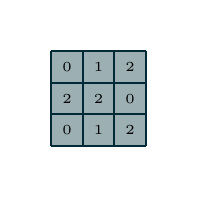
\begin{tikzpicture}[scale=.4,every node/.style={minimum size=1cm}, on grid]
            \draw[fill=base02,opacity=0.4] (0,0) rectangle (3,3);
            \draw[draw=base03,thick] (0,0) grid (3,3);
            \node (00) at (0.5,2.5) {\tiny 0};
            \node (01) at (1.5,2.5) {\tiny 1};
            \node (02) at (2.5,2.5) {\tiny 2};
            \node (10) at (0.5,1.5) {\tiny 2};
            \node (11) at (1.5,1.5) {\tiny 2};
            \node (12) at (2.5,1.5) {\tiny 0};
            \node (20) at (0.5,0.5) {\tiny 0};
            \node (21) at (1.5,0.5) {\tiny 1};
            \node (22) at (2.5,0.5) {\tiny 2};
    \end{tikzpicture}
\end{figure}

\begin{figure}[p]
    \centering
    \includegraphics[width=0.32\textwidth]{pdf/numerical_no_padding_no_strides_00.pdf}
    \includegraphics[width=0.32\textwidth]{pdf/numerical_no_padding_no_strides_01.pdf}
    \includegraphics[width=0.32\textwidth]{pdf/numerical_no_padding_no_strides_02.pdf}
    \includegraphics[width=0.32\textwidth]{pdf/numerical_no_padding_no_strides_03.pdf}
    \includegraphics[width=0.32\textwidth]{pdf/numerical_no_padding_no_strides_04.pdf}
    \includegraphics[width=0.32\textwidth]{pdf/numerical_no_padding_no_strides_05.pdf}
    \includegraphics[width=0.32\textwidth]{pdf/numerical_no_padding_no_strides_06.pdf}
    \includegraphics[width=0.32\textwidth]{pdf/numerical_no_padding_no_strides_07.pdf}
    \includegraphics[width=0.32\textwidth]{pdf/numerical_no_padding_no_strides_08.pdf}
    \caption{\label{fig:numerical_no_padding_no_strides} 计算离散卷积的输出值.}
\end{figure}

\begin{figure}[p]
    \centering
    \includegraphics[width=0.32\textwidth]{pdf/numerical_padding_strides_00.pdf}
    \includegraphics[width=0.32\textwidth]{pdf/numerical_padding_strides_01.pdf}
    \includegraphics[width=0.32\textwidth]{pdf/numerical_padding_strides_02.pdf}
    \includegraphics[width=0.32\textwidth]{pdf/numerical_padding_strides_03.pdf}
    \includegraphics[width=0.32\textwidth]{pdf/numerical_padding_strides_04.pdf}
    \includegraphics[width=0.32\textwidth]{pdf/numerical_padding_strides_05.pdf}
    \includegraphics[width=0.32\textwidth]{pdf/numerical_padding_strides_06.pdf}
    \includegraphics[width=0.32\textwidth]{pdf/numerical_padding_strides_07.pdf}
    \includegraphics[width=0.32\textwidth]{pdf/numerical_padding_strides_08.pdf}
    \caption{\label{fig:numerical_padding_strides} 对 $N = 2$, $i_1 = i_2 = 5$, $k_1 = k_2 = 3$, $s_1 = s_2 = 2$, 和 $p_1 = p_2 = 1$ 计算离散卷积的输出值.}
\end{figure}


\noindent 并对结果进行求和. 可以用不同的卷积核重复该过程,以生成所需的输出特征映射  (\autoref{fig:full_picture}). 这个过程的最终输出被称为 {\em 输出特征映射} (output feature maps). \footnote{%
    虽然从信号处理的角度来看,卷积和交叉相关是有区别的,但当学习了卷积核时,两者就可以互换了. 为了简单起见,以及与大多数机器学习文献保持一致,我们将在这个指南中使用 {\em 卷积\/}(convolution) 这一术语.}

如果有多个输入特征映射,则核必须是三维的——或者等价于每个特征映射都用一个不同的核进行卷积,并且生成的特征映射主元素相加,以生成输出特征映射。

卷积(见图\autoref{fig:numerical_no_padding_no_strides})是二维卷积的一种形式,但是它可以生成N维卷积. 例如,在三维卷积中,卷积核可以是一个{\em 立方体\/} (cuboid),而且会在输入特征映射的的高度、宽度和深度上滑动. 

定义了一批离散卷积的核有一个形状对应$(n, m, k_1, \ldots, k_N)$的某个排列,其中

\begin{equation*}
\begin{split}
    n &\equiv \text{输出特征映射的数量},\\
    m &\equiv \text{输入特征映射的数量},\\
    k_j &\equiv \text{沿 $j$ 轴核的尺寸}.
\end{split}
\end{equation*}

以下属性会影响沿$j$轴方向卷积层的输出尺寸$o_j$ : 
\begin{itemize}
    \item $i_j$: 沿 $j$轴的输入尺寸,
    \item $k_j$: 沿 $j$轴的核尺寸,
    \item $s_j$: 沿$j$轴的步长 (核的两个连续位置之间的距离),
    \item $p_j$: 沿$j$轴方向的零填充 (在轴开始和结尾处连接的$0$的数目).
\end{itemize}

\noindent 例如, \autoref{fig:numerical_padding_strides} 展示了一个应用于$5 \times 5$输入的 $3
\times 3$ 卷积核,使用了 $2 \times 2$ 的步长填充了$1\times 1$的零边界.

注意,步长构成了一种 \emph{子采样}(subsampling) 形式. 步长作为衡量核被翻译多少的一种替代方法,它也可以看作保留了多少输出. 例如,以两个跃点移动卷积核相当于以一个跃点移动卷积核,但只保留奇数个输出元素 (\autoref{fig:strides_subsampling}).

\begin{figure}[p]
    \centering
    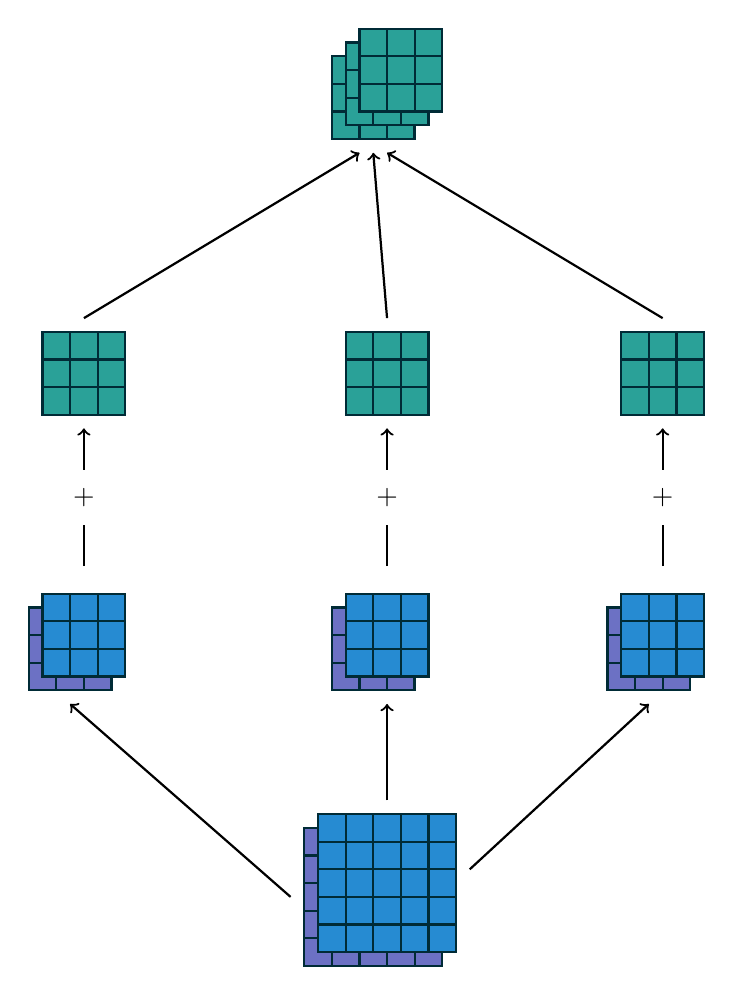
\begin{tikzpicture}[scale=.35,every node/.style={minimum size=1cm}, on grid]
        \begin{scope}[xshift=0cm,yshift=0cm]
            \begin{scope}[xshift=0cm,yshift=0cm]
                \draw[draw=base03,fill=violet,thick]
                    (0,0) grid (5,5) rectangle (0,0);
            \end{scope}
            \begin{scope}[xshift=0.5cm,yshift=0.5cm]
                \draw[draw=base03,fill=blue,thick]
                    (0,0) grid (5,5) rectangle (0,0);
            \end{scope}
        \end{scope}
        \foreach \x in {-10,1,11} {%
            \begin{scope}[xshift=\x cm,yshift=10cm]
                \begin{scope}[xshift=0cm,yshift=0cm]
                    \draw[draw=base03,fill=violet,thick]
                        (0,0) grid (3,3) rectangle (0,0);
                \end{scope}
                \begin{scope}[xshift=0.5cm,yshift=0.5cm]
                    \draw[draw=base03,fill=blue,thick]
                        (0,0) grid (3,3) rectangle (0,0);
                \end{scope}
            \end{scope}
            \begin{scope}[xshift=\x cm,yshift=20cm]\begin{scope}[xshift=0.5cm]
                \draw[draw=base03,fill=cyan,thick]
                    (0,0) grid (3,3) rectangle (0,0);
            \end{scope}\end{scope}
        }
        \begin{scope}[xshift=1cm,yshift=30cm]
            \foreach \s in {0.0,0.5,1.0} {%
                \begin{scope}[xshift=\s cm,yshift=\s cm]
                    \draw[draw=base03,fill=cyan,thick]
                        (0,0) grid (3,3) rectangle (0,0);
                \end{scope}
            }
        \end{scope}
        \draw[->, thick] (-0.5,2.5) to (-8.5,9.5);
        \draw[->, thick] (3,6) to (3,9.5);
        \draw[->, thick] (6,3.5) to (12.5,9.5);
        \draw[thick]  (-8,14.5) to (-8,16);
        \draw[->, thick]  (-8,18) to (-8,19.5);
        \node[thick] (p1) at (-8,17) {$+$};
        \draw[thick]  (3,14.5) to (3,16);
        \draw[->, thick]  (3,18) to (3,19.5);
        \node[thick] (p2) at (3,17) {$+$};
        \draw[thick]  (13,14.5) to (13,16);
        \draw[->, thick]  (13,18) to (13,19.5);
        \node[thick] (p3) at (13,17) {$+$};
        \draw[->, thick]  (-8,23.5) to (2,29.5);
        \draw[->, thick]  (3,23.5) to (2.5,29.5);
        \draw[->, thick]  (13,23.5) to (3,29.5);
    \end{tikzpicture}
    \caption{\label{fig:full_picture} 一种从两个输入特征映射到三个输出特征映射的卷积映射,使用$3 \times 2 \times 3 \times 3$的一批卷积核$\mathbf{w}$. 在左边的路径中,输入特征映射 1 与核 $\mathbf{w}_{1,1}$ 做卷积且输入特征映射 2 与核 $\mathbf{w}_{1,2}$做卷积,并将结果逐元素相加,形成第一个输出特征映射. 对中间和右侧的路径重复相同的步骤,以形成第二和第三个特征映射,并将所有的三个输出特征映射组合在一起形成输出.}
\end{figure}

\begin{figure}[p]
    \centering
    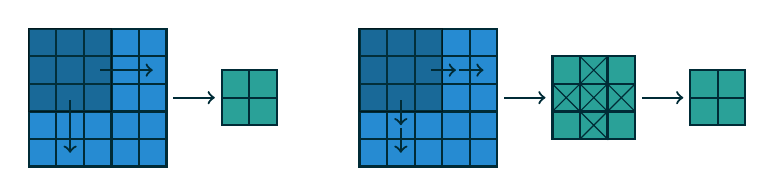
\begin{tikzpicture}[scale=.35,every node/.style={minimum size=1cm}, on grid]
        \begin{scope}[xshift=0,yshift=0cm]
            \begin{scope}[xshift=0cm,yshift=0cm]
                \draw[draw=base03,fill=blue,thick] (0,0) grid (5,5) rectangle (0,0);
                \draw[fill=base02, opacity=0.4] (0,2) rectangle (3,5);
            \end{scope}
            \begin{scope}[xshift=7cm,yshift=1.5cm]
                \draw[draw=base03,fill=cyan,thick] (0,0) grid (2,2) rectangle (0,0);
            \end{scope}
        \end{scope}
        \draw[draw=base03, ->, thick] (2.6,3.5) to  (4.5,3.5);
        \draw[draw=base03, ->, thick] (1.5,2.4) to (1.5,0.5);
        \draw[draw=base03, ->, thick] (5.25, 2.5) to (6.75, 2.5);
        \begin{scope}[xshift=12cm,yshift=0cm]
            \begin{scope}[xshift=0cm,yshift=0cm]
                \draw[draw=base03,fill=blue,thick] (0,0) grid (5,5) rectangle (0,0);
                \draw[fill=base02, opacity=0.4] (0,2) rectangle (3,5);
            \end{scope}
            \begin{scope}[xshift=7cm,yshift=1cm]
                \draw[draw=base03,fill=cyan,thick] (0,0) grid (3,3) rectangle (0,0);
                \draw[draw=base03] (1,0) -- (2,1) -- (2,0) -- (1,1);
                \draw[draw=base03] (0,1) -- (1,2) -- (1,1) -- (0,2);
                \draw[draw=base03] (1,1) -- (2,2) -- (2,1) -- (1,2);
                \draw[draw=base03] (2,1) -- (3,2) -- (3,1) -- (2,2);
                \draw[draw=base03] (1,2) -- (2,3) -- (2,2) -- (1,3);
            \end{scope}
            \begin{scope}[xshift=12cm,yshift=1.5cm]
                \draw[draw=base03,fill=cyan,thick] (0,0) grid (2,2) rectangle (0,0);
            \end{scope}
        \end{scope}
        \draw[draw=base03, ->, thick] (14.6,3.5) to  (15.5,3.5);
        \draw[draw=base03, ->, thick] (15.6,3.5) to  (16.5,3.5);
        \draw[draw=base03, ->, thick] (13.5,2.4) to (13.5,1.5);
        \draw[draw=base03, ->, thick] (13.5,1.4) to (13.5,0.5);
        \draw[draw=base03, ->, thick] (17.25, 2.5) to (18.75, 2.5);
        \draw[draw=base03, ->, thick] (22.25, 2.5) to (23.75, 2.5);
    \end{tikzpicture}
    \caption{\label{fig:strides_subsampling} 另一种步长可视方法. 不是以$s = 2$ (左边)的增量去转换 $3 \times 3$ 的卷积核,而是以 $1$ 为增量进行转换,且只保留一个 $s = 2$ 的输出元素(右边).}
\end{figure}

\section{池化}

除了离散卷积本身, {\em 池化\/} (pooling) 操作是构成卷积神经网络的另一个重要部分. 池化操作通过使用某种函数来汇总子区域,例如取平均值或最大值,以此减少特征映射的大小.

池化的工作原理是在输入中滑动一个窗口,并将窗口的内容提供给 {\em 池化函数} (pooling function). 从某种意义上讲,池化的工作原理与离散卷积十分类似,但它用其他函数代替了卷积核形成的线性组合. \autoref{fig:numerical_average_pooling}
给出了一个平均池化的例子, 而 \autoref{fig:numerical_max_pooling}
给出了最大值池化的例子.

以下属性会影响沿$j$轴池化层的输出大小$o_j$: 

\begin{itemize}
    \item $i_j$: 沿$j$轴的输入尺寸,
    \item $k_j$: 沿$j$轴的池化窗口大小,
    \item $s_j$: 沿$j$轴的步长 (池化窗口的两连续位置之间的距离).
\end{itemize}

\begin{figure}[p]
    \centering
    \includegraphics[width=0.32\textwidth]{pdf/numerical_average_pooling_00.pdf}
    \includegraphics[width=0.32\textwidth]{pdf/numerical_average_pooling_01.pdf}
    \includegraphics[width=0.32\textwidth]{pdf/numerical_average_pooling_02.pdf}
    \includegraphics[width=0.32\textwidth]{pdf/numerical_average_pooling_03.pdf}
    \includegraphics[width=0.32\textwidth]{pdf/numerical_average_pooling_04.pdf}
    \includegraphics[width=0.32\textwidth]{pdf/numerical_average_pooling_05.pdf}
    \includegraphics[width=0.32\textwidth]{pdf/numerical_average_pooling_06.pdf}
    \includegraphics[width=0.32\textwidth]{pdf/numerical_average_pooling_07.pdf}
    \includegraphics[width=0.32\textwidth]{pdf/numerical_average_pooling_08.pdf}
    \caption{\label{fig:numerical_average_pooling} 使用$1 \times 1$步长计算$5 \times 5$输入、$3 \times 3$平均池化操作的输出值.}
\end{figure}

\begin{figure}[p]
    \centering
    \includegraphics[width=0.32\textwidth]{pdf/numerical_max_pooling_00.pdf}
    \includegraphics[width=0.32\textwidth]{pdf/numerical_max_pooling_01.pdf}
    \includegraphics[width=0.32\textwidth]{pdf/numerical_max_pooling_02.pdf}
    \includegraphics[width=0.32\textwidth]{pdf/numerical_max_pooling_03.pdf}
    \includegraphics[width=0.32\textwidth]{pdf/numerical_max_pooling_04.pdf}
    \includegraphics[width=0.32\textwidth]{pdf/numerical_max_pooling_05.pdf}
    \includegraphics[width=0.32\textwidth]{pdf/numerical_max_pooling_06.pdf}
    \includegraphics[width=0.32\textwidth]{pdf/numerical_max_pooling_07.pdf}
    \includegraphics[width=0.32\textwidth]{pdf/numerical_max_pooling_08.pdf}
    \caption{\label{fig:numerical_max_pooling} 使用$1 \times 1$步长计算$5 \times 5$输入、$3 \times 3$最大值池化操作的输出值.}
\end{figure}

\chapter{卷积运算}

卷积层属性之间的关系分析起来很容易,因为它们不跨轴交互,即沿$j$轴选定的卷积核大小、步长和零填充只影响$j$轴的输出大小. 因此,本章将重点介绍以下的简化设置:

\begin{itemize}
    \item 二维离散卷积 ($N = 2$),
    \item 方形输入 ($i_1 = i_2 = i$),
    \item 方形核尺寸 ($k_1 = k_2 = k$),
    \item 沿着两轴的相同步长 ($s_1 = s_2 = s$),
    \item 沿着两轴的相同零填充 ($p_1 = p_2 = p$).
\end{itemize}

这有助于分析及可视化,但请记住,这里概述的结果也可推广到N维和非方形情形.

\section{无零填充,单位步长}

要分析的最简单情形是卷积核在输入(即 $s = 1$ 且 $p = 0$时)的每个位置滑动.
\autoref{fig:no_padding_no_strides} 提供了当 $i = 4$ 且 $k =
3$ 时的例子.

在这种情况下,定义输出大小的一种方法是确定在输入层上可放置卷积核的个数. 让我们考虑宽度轴:内核从输入特征映射的最左边开始,一步步滑动,直到它接触输入的右侧. 输出的大小等于所执行步数加一,即内核的初始位置 (\autoref{fig:no_padding_no_strides_explained}). 相同的逻辑应用于高度轴.

更正式地说,可以推断出以下关系:

\begin{relationship}\label{rel:no_padding_no_strides}
对任何 $i$ 和 $k$, 以及 对 $s = 1$ 和 $p = 0$,
\begin{equation*}
    o = (i - k) + 1.
\end{equation*}
\end{relationship}

\begin{figure}[p]
    \centering
    \includegraphics[width=0.24\textwidth]{pdf/no_padding_no_strides_00.pdf}
    \includegraphics[width=0.24\textwidth]{pdf/no_padding_no_strides_01.pdf}
    \includegraphics[width=0.24\textwidth]{pdf/no_padding_no_strides_02.pdf}
    \includegraphics[width=0.24\textwidth]{pdf/no_padding_no_strides_03.pdf}
    \caption{\label{fig:no_padding_no_strides} (无零填充,单位步长)
    用单位步长(即 $i = 4$, $k = 3$, $s = 1$ 和 $p = 0$),将 $3 \times 3$ 的卷积核与 $4 \times 4$ 的输入做卷积.}
\end{figure}

\begin{figure}[p]
    \centering
    \includegraphics[width=0.24\textwidth]{pdf/arbitrary_padding_no_strides_00.pdf}
    \includegraphics[width=0.24\textwidth]{pdf/arbitrary_padding_no_strides_01.pdf}
    \includegraphics[width=0.24\textwidth]{pdf/arbitrary_padding_no_strides_02.pdf}
    \includegraphics[width=0.24\textwidth]{pdf/arbitrary_padding_no_strides_03.pdf}
    \caption{\label{fig:arbitrary_padding_no_strides} (任意填充, 单位步长) 用单位步长(即 $i = 5$, $k = 4$, $s = 1$ 和 $p = 2$),将 $4 \times 4$ 的卷积核与 $5 \times 5$的输入做卷积,并用$2 \times 2$的零边界填充.}
\end{figure}

\begin{figure}[p]
    \centering
    \includegraphics[width=0.24\textwidth]{pdf/same_padding_no_strides_00.pdf}
    \includegraphics[width=0.24\textwidth]{pdf/same_padding_no_strides_01.pdf}
    \includegraphics[width=0.24\textwidth]{pdf/same_padding_no_strides_02.pdf}
    \includegraphics[width=0.24\textwidth]{pdf/same_padding_no_strides_03.pdf}
    \caption{\label{fig:same_padding_no_strides} (半填充, 单位步长)
    用半填充和单位步长(即 $i = 5$, $k = 3$, $s = 1$ 和 $p = 2$),将 $3 \times 3$ 的卷积核与 $5 \times 5$ 的输入做卷积.}
\end{figure}

\begin{figure}[p]
    \centering
    \includegraphics[width=0.24\textwidth]{pdf/full_padding_no_strides_00.pdf}
    \includegraphics[width=0.24\textwidth]{pdf/full_padding_no_strides_01.pdf}
    \includegraphics[width=0.24\textwidth]{pdf/full_padding_no_strides_02.pdf}
    \includegraphics[width=0.24\textwidth]{pdf/full_padding_no_strides_03.pdf}
    \caption{\label{fig:full_padding_no_strides} (全填充,单位步长)
    使用全填充和单位步长(即 $i = 5$, $k = 3$, $s = 1$ 和 $p = 2$),将 $3 \times 3$ 的卷积核与 $5 \times 5$ 的输入做卷积.}
\end{figure}

\section{有零填充,单位步长}

为了考虑零填充(即仅限于$s = 1$), 让我们考虑其对有效输入大小的影响: 使用 $p$ 零填充将有效输入大小从 $i$ 改为 $i + 2p$. 在一般情况下,
\autoref{rel:no_padding_no_strides} 可推出以下关系:

\begin{relationship}\label{rel:arbitrary_padding_no_strides}
对任何 $i$, $k$ 和 $p$, 且对 $s = 1$,有
\begin{equation*}
    o = (i - k) + 2p + 1.
\end{equation*}
\end{relationship}

\noindent \autoref{fig:arbitrary_padding_no_strides} 给出了当 $i
= 5$, $k = 4$ 且 $p = 2$时的一个例子.

实际上,零填充的两个特定实例由于各自的性质而被广泛使用. 让我们更详细地讨论一下.

\subsection{半填充(相似填充)}

输出大小和输入大小相同 (即 $o = i$) 是一个理想的性质:

\begin{relationship}\label{rel:same_padding_no_strides}
对任何 $i$ 和奇数 $k$ ($k = 2n + 1, \quad n \in \mathbb{N}$), $s = 1$, $p = \lfloor k / 2 \rfloor = n$, 有
\begin{equation*}
\begin{split}
    o &= i + 2 \lfloor k / 2 \rfloor - (k - 1) \\
      &= i + 2n - 2n \\
      &= i.
\end{split}
\end{equation*}
\end{relationship}

\noindent 这有时被称为 {\em 半填充\/} (或 {\em 相似填充\/}). \autoref{fig:same_padding_no_strides} 给出了当
$i = 5$, $k = 3$ 且 (因此) $p = 1$ 时的一个例子.

\subsection{全填充}

虽然对一个核做卷积时,通常会 {\em 减小\/} 相对于输入的输出大小,但有时需要相反的结果. 这可以通过适当的零填充来实现:

\begin{relationship}\label{rel:full_padding_no_strides}
对任何 $i$ 和 $k$, 且对 $p = k - 1$ 和 $s = 1$, 有
\begin{equation*}
\begin{split}
    o &= i + 2(k - 1) - (k - 1) \\
      &= i + (k - 1).
\end{split}
\end{equation*}
\end{relationship}

\noindent 这有时被称为 {\em 全} 填充, 因为在这个设定中,输入特征映射上卷积核的每一个可能的部分或完全重叠都被考虑在内. \autoref{fig:full_padding_no_strides}
给出了当 $i = 5$, $k = 3$ 且 (因此) $p = 2$ 的一个例子.

\section{无零填充,非单位步长}

迄今为止导出的所有关系仅适用于单位步长卷积. 合并非单位步长需要另一种进一步的推理. 为了便于分析,让我们暂时忽略零填充 (即$s > 1$
且 $p = 0$). \autoref{fig:no_padding_strides} 给出了当 $i =
5$, $k = 3$ 且 $s = 2$ 时的一个例子.

同样,输出大小可以根据卷积核在输入上的可能位置的数量来定义. 让我们考虑宽度轴:卷积核像往常一样从输入的最左边开始,但是这次它以大小为 $s$ 滑动,直到它接触到输入的右侧. 这个输出的大小再次等于所执行的步骤数加一,说明了卷积核的初始位置 
(\autoref{fig:no_padding_strides_explained}). 相同的逻辑应用于高度轴.

由此可以推断出以下关系:

\begin{relationship}\label{rel:no_padding_strides}
对任何 $i$, $k$ 和 $s$, 并对 $p = 0$,有
\begin{equation*}
    o = \left\lfloor \frac{i - k}{s} \right\rfloor + 1.
\end{equation*}
\end{relationship}

\noindent 下取整函数说明了这样一个事实:有时最后可能的步骤与到达输入层末尾的卷积核 {\em 不\/} 一致, 也就是说, 一些输入单元被忽略了 (关于这种情况,参见 \autoref{fig:padding_strides_odd} ).

\section{有零填充,非单位步长}

最一般的情况(使用非单位步长在零填充的输入上做卷积)可以通过在大小为$i + 2p$的有效输入上应用 \autoref{rel:no_padding_strides} 来推导,类似于 \autoref{rel:arbitrary_padding_no_strides} 所做的工作: 

\begin{relationship}\label{rel:padding_strides}
对任何 $i$, $k$, $p$ 和 $s$,
\begin{equation*}
    o = \left\lfloor \frac{i + 2p - k}{s} \right\rfloor + 1.
\end{equation*}
\end{relationship}

\noindent 如前所述,下取整函数意味着在某些情况下,卷积将为多个输入大小生成相同的输出大小. 更具体地讲,如果 $i + 2p - k$ 是 $s$ 的倍数, 所有输出大小 $j = i + a, \quad a
\in \{0,\ldots,s - 1\}$ 都将产生相同的输出大小. 注意,这种二义性仅应用于 $s > 1$.

\autoref{fig:padding_strides} 给出了当 $i = 5$, $k = 3$, $s = 2$
和 $p = 1$ 时的一个例子, 而 \autoref{fig:padding_strides_odd} 给出了当 $i = 6$, $k = 3$, $s = 2$ 且 $p = 1$ 时的例子. 有趣的是,尽管输入大小不同,这些卷积依然共享同一输出大小. 虽然这不影响{\em 卷积}(convolutions) 的分析,但这将使{\em 转置卷积} (transposed convolutions) 的分析复杂化.

\begin{figure}[p]
    \centering
    \includegraphics[width=0.24\textwidth]{pdf/no_padding_strides_00.pdf}
    \includegraphics[width=0.24\textwidth]{pdf/no_padding_strides_01.pdf}
    \includegraphics[width=0.24\textwidth]{pdf/no_padding_strides_02.pdf}
    \includegraphics[width=0.24\textwidth]{pdf/no_padding_strides_03.pdf}
    \caption{\label{fig:no_padding_strides} (无零填充,任意步长) 
    使用 $2 \times 2$ 步长 (即 $i = 5$, $k = 3$, $s = 2$ 和 $p = 0$) 将 $3 \times 3$ 的卷积核与 $5 \times 5$ 的输入做卷积.}
\end{figure}

\begin{figure}[p]
    \centering
    \includegraphics[width=0.24\textwidth]{pdf/padding_strides_00.pdf}
    \includegraphics[width=0.24\textwidth]{pdf/padding_strides_01.pdf}
    \includegraphics[width=0.24\textwidth]{pdf/padding_strides_02.pdf}
    \includegraphics[width=0.24\textwidth]{pdf/padding_strides_03.pdf}
    \caption{\label{fig:padding_strides} (任意填充和步长)
    使用$2 \times 2$ 步长 (即 $i = 5$, $k = 3$, $s = 2$ 和 $p = 1$) 将 $3 \times 3$ 的卷积核与填充了$1 \times 1$零边界的 $5 \times 5$ 输入做卷积. }
\end{figure}

\begin{figure}[p]
    \centering
    \includegraphics[width=0.24\textwidth]{pdf/padding_strides_odd_00.pdf}
    \includegraphics[width=0.24\textwidth]{pdf/padding_strides_odd_01.pdf}
    \includegraphics[width=0.24\textwidth]{pdf/padding_strides_odd_02.pdf}
    \includegraphics[width=0.24\textwidth]{pdf/padding_strides_odd_03.pdf}
    \caption{\label{fig:padding_strides_odd} (任意填充和步长)
    使用$2 \times 2$ 步长(即 $i = 6$, $k = 3$, $s = 2$ 且 $p = 1$)在 $6 \times 6$ 的输入上与 $3 \times 3$的卷积核做卷积,输入使用 $2 \times 2$ 的步长,并填充 $1 \times 1$ 的零边界. 在这个例子中,零填充的底行和右列不被卷积核覆盖.}
\end{figure}

\begin{figure}[p]
    \centering
    \begin{subfigure}[t]{0.48\textwidth}
        \centering
        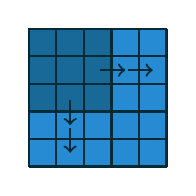
\begin{tikzpicture}[scale=.35,every node/.style={minimum size=1cm},
                            on grid]
            \draw[fill=blue] (0,0) rectangle (5,5);
            \draw[draw=base03, thick] (0,0) grid (5,5);
            \draw[fill=base02, opacity=0.4] (0,2) rectangle (3,5);
            \draw[step=10mm, base03, thick] (0,2) grid (3,5);
            \draw[draw=base03, ->, thick] (2.6,3.5) to  (3.5,3.5);
            \draw[draw=base03, ->, thick] (3.6,3.5) to  (4.5,3.5);
            \draw[draw=base03, ->, thick] (1.5,2.4) to  (1.5,1.5);
            \draw[draw=base03, ->, thick] (1.5,1.4) to  (1.5,0.5);
        \end{tikzpicture}
        \caption{\label{fig:no_padding_no_strides_explained} 卷积核必须向右滑动两步才能接触到输入的右侧(等价于向下). 加一以说明初始卷积核位置,输出大小为 $3 \times 3$.}
    \end{subfigure}
    ~
    \begin{subfigure}[t]{0.48\textwidth}
        \centering
        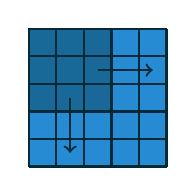
\begin{tikzpicture}[scale=.35,every node/.style={minimum size=1cm},
                            on grid]
            \draw[fill=blue] (0,0) rectangle (5,5);
            \draw[draw=base03, thick] (0,0) grid (5,5);
            \draw[fill=base02, opacity=0.4] (0,2) rectangle (3,5);
            \draw[step=10mm, base03, thick] (0,2) grid (3,5);
            \draw[draw=base03, ->, thick] (2.5,3.5) to  (4.5,3.5);
            \draw[draw=base03, ->, thick] (1.5,2.5) to  (1.5,0.5);
        \end{tikzpicture}
        \caption{\label{fig:no_padding_strides_explained} 
        内核必须向右滑动一步(大小为2)才能接触到输入的右侧(相当于向下). 加一以说明初始卷积核的位置,输出大小为 $2 \times 2$.}
    \end{subfigure}
    \caption{计算卷积核位置.}
\end{figure}

\chapter{池化运算}

在神经网络中,池化层对输入的微小转换满足不变性. 最常见的一种池化是\emph{最大值池化}(max pooling),它包括将输入拆分为(通常不重叠)块并输出每个块的最大值. 其他类型的池化也存在,例如平均值池化,它们都具有相同的思想,即通过对某些块应用非线性来汇总局部输入 \citep{%
boureau-cvpr-10,boureau-icml-10,boureau-iccv-11,ICML2011Saxe_551}.

一些读者可能已经注意到,卷积运算的处理仅仅依赖于一个假设,即某些函数被重复应用到输入的子集上. 这意味着上一章中导出的关系可以在池化算法下重用. 由于池化不涉及零填充,描述一般情况的关系如下: 

\begin{relationship}\label{rel:pooling}
对任何 $i$, $k$ 和 $s$, 有
\begin{equation*}
    o = \left\lfloor \frac{i - k}{s} \right\rfloor + 1.
\end{equation*}
\end{relationship}

\noindent 这种关系适用于任何类型的池化.

\chapter{转置卷积运算}

转置卷积用于与正常卷积做相反方向变换的情况,即从具有某种卷积输出形状到具有其输入形状的情况,同时保持与所述卷积兼容的连接模式. 例如,可以使用这样的转换作为卷积自动编码器的解码层,或者将特征映射投影到更高维空间.

同样,卷积的情况比全连接的情况复杂得多,后者只需要使用形状被转置的权重矩阵. 然而,由于每一个卷积都可以归结为一个矩阵运算的有效实现,因此从全连接情形中获得的见解对于解决卷积情形是有用的.

与卷积算法一样,转置卷积算法的论文由于转置卷积不跨轴交互的性质而得以简化.

本章将着重于以下设定:

\begin{itemize}
    \item 2维转置卷积 ($N = 2$),
    \item 方形输入 ($i_1 = i_2 = i$),
    \item 方形核大小 ($k_1 = k_2 = k$),
    \item 沿着两轴的相同步长 ($s_1 = s_2 = s$),
    \item 沿着两轴的相同零填充 ($p_1 = p_2 = p$).
\end{itemize}

\noindent 结果将再次推广到$N$维的情形.

\section{作为矩阵运算的卷积}

以 \autoref{fig:no_padding_no_strides} 表示的卷积为例. 如果输入和输出从左至右、从上到下展开为向量,卷积可以表示为稀疏矩阵 $\mathbf{C}$ ,其中非零元素是卷积核的元素 $w_{i,j}$  ($i$ 和 $j$ 分别是卷积核的行和列):
\begin{equation*}
\resizebox{.98\hsize}{!}{$
    \begin{pmatrix}
    w_{0,0} & w_{0,1} & w_{0,2} & 0       & w_{1,0} & w_{1,1} & w_{1,2} & 0       &
    w_{2,0} & w_{2,1} & w_{2,2} & 0       & 0       & 0       & 0       & 0       \\
    0       & w_{0,0} & w_{0,1} & w_{0,2} & 0       & w_{1,0} & w_{1,1} & w_{1,2} &
    0       & w_{2,0} & w_{2,1} & w_{2,2} & 0       & 0       & 0       & 0       \\
    0       & 0       & 0       & 0       & w_{0,0} & w_{0,1} & w_{0,2} & 0       &
    w_{1,0} & w_{1,1} & w_{1,2} & 0       & w_{2,0} & w_{2,1} & w_{2,2} & 0       \\
    0       & 0       & 0       & 0       & 0       & w_{0,0} & w_{0,1} & w_{0,2} &
    0       & w_{1,0} & w_{1,1} & w_{1,2} & 0       & w_{2,0} & w_{2,1} & w_{2,2} \\
    \end{pmatrix}$}
\end{equation*}

此线性运算将展平后的输入矩阵作为16维向量,并生成一个4维向量,该向量随后变为形状是 $2 \times 2$ 的输出矩阵.

使用这种表示方法,通过转置$\mathbf{C}$很容易得到反向传递; 换句话说,通过将损失乘以 $\mathbf{C}^T$,可以反向传播误差. 这一操作以一个4维向量作为输入,生成一个16维向量作为输出,并且其连接模式通过一定的构造与 $\mathbf{C}$ 兼容.

值得注意的是,卷积核 $\mathbf{w}$ 定义了用于向前和向后传递的矩阵 $\mathbf{C}$ 和
$\mathbf{C}^T$ .

\section{转置卷积}

现在让我们考虑一下从4维空间映射到16维空间,并同时保持\autoref{fig:no_padding_no_strides}中描述的卷积连接模式反过来又需要什么? 这一操作称为 {\em 转置卷积} (transposed convolution).

转置卷积也叫 {\em 分步卷积\/}(fractionally strided convolutions)
或 {\em 逆卷积\/}(deconvolutions)\footnote{ ``逆卷积''(deconvolution) 一词有时在文献中使用,但我们不推荐这样用,理由是逆卷积在数学上被定义为卷积的逆,它不同于转置卷积.},通过交换卷积的前向和反向传递来工作. 一种说法是卷积核定义了一个卷积,但它是直接卷积还是转置卷积取决于前向和反向传递的计算方式.

例如, 虽然卷积核 $\mathbf{w}$ 定义了一个卷积,其正向和反向传播分别通过与 $\mathbf{C}$ 和 $\mathbf{C}^T$ 相乘来计算,但它 {\em 也} 定义了一个转置的卷积,其正向和反向传递分别通过与 $\mathbf{C}^T$ 和 $(\mathbf{C}^T)^T = \mathbf{C}$ 相乘来计算.\footnote{转置卷积操作可以被认为是{\em 某些}卷积相对于其输入的梯度,这通常是转置卷积在实际应用中的实现方式.}

最后要注意的是,我们总是可以用直接卷积来模拟转置卷积. 缺点是,它通常需要向输入中添加许多列和零行,导致实现效率大大降低.

在目前所介绍的基础上,本章将从卷积算法一章开始,通过引用与其共享卷积核的直接卷积来推导每个转置卷积的性质,并定义等效的直接卷积.

\section{无零填充,单位步长,转置}

考虑给定输入上转置卷积的最简单方法,是将这种输入想象为应用于某些初始特征映射的直接卷积的结果. 因此,卷积可以看作是恢复初始特征映射 \emph{形状}(shape)~\footnote{注意到转置卷积并不保证恢复输入本身,因为它不是定义为卷积的逆,而是返回具有相同宽度和高度的特征映射.} 的操作.

考虑在单位步长且无填充的$4 \times 4$输入(即 $i = 4$, $k = 3$, $s = 1$ 且 $p = 0$)上应用 $3 \times 3$ 的卷积核 . 就像 \autoref{fig:no_padding_no_strides}中描述的那样,这产生了一个 $2 \times 2$ 的输出. 当应用于$2 \times 2$的输入时,这个卷积的转置将产生形状为 $4 \times 4$ 的输出.

另一种获得转置卷积结果的方法是应用一个等价(但效率要低得多)的直接卷积. 到目前为止描述的例子可以通过使用单位步长(即 $i' = 2$, $k' = k$, $s' = 1$ 且 $p' = 2$)将 $3 \times 3$ 的卷积核与一个 $2 \times 2$ 的输入做卷积,这个输入使用单位步长且填充了 $2 \times 2$ 的零边界,如\autoref{fig:no_padding_no_strides_transposed} 展示的那样. 值得注意的是,卷积核和步长的大小保持不变,但是转置卷积的输入现在是零填充.\footnote{注意,尽管相当于应用转置矩阵,但这种以补零的形式可视化添加了大量的零乘法. 这里这样做是为了说明问题,但是效率低下,软件实现通常不会执行无用的零乘法.}

理解零填充背后逻辑的一个方法是考虑转置卷积的连接模式,并用它来指导等效卷积的设计. 例如,直接卷积输入的左上角像素只贡献给输出的左上角像素,右上角像素只连接到右上角的输出像素等.

为了在等价的卷积中保持相同的连接模式,有必要对输入进行零填充,使卷积核的第一个(左上)应用只接触左上角像素,即填充必须等于核的大小减1.

以同样的方式进行,可以确定图像其他元素类似的观察结果,从而得到以下关系:

\begin{relationship}\label{rel:no_padding_no_strides_transposed}
由 $s = 1$, $p = 0$ 和 $k$ 描述的卷积具有由 $k' = k$, $s' = s$ 和 $p' = k - 1$ 描述的相关转置卷积,并且其输入大小为 
\begin{equation*}
    o' = i' + (k - 1).
\end{equation*}
\end{relationship}

有趣的是,这对应于单位步长的全填充卷积.

\section{有零填充,单位步长,转置}

已知无填充卷积的转置等价于对一个零填充输入做卷积,就可以合理地假设零填充卷积的转置等价于对{\em 较少}的零填充输入做卷积.

确实如此,对 $i = 5$, $k = 4$ 和 $p = 2$,如 \autoref{fig:arbitrary_padding_no_strides_transposed} 所示.

在形式上,以下关系适用于零填充卷积:

\begin{relationship}\label{rel:arbitrary_padding_no_strides_transposed}
一个由 $s = 1$, $k$ 和 $p$ 描述的卷积与一个由 $k' = k$, $s' = s$ 和 $p' = k -
p - 1$ 描述的转置卷积相关联. 且其输出大小为
\begin{equation*}
    o' = i' + (k - 1) - 2p.
\end{equation*}
\end{relationship}

\begin{figure}[p]
    \centering
    \includegraphics[width=0.24\textwidth]{pdf/no_padding_no_strides_transposed_00.pdf}
    \includegraphics[width=0.24\textwidth]{pdf/no_padding_no_strides_transposed_01.pdf}
    \includegraphics[width=0.24\textwidth]{pdf/no_padding_no_strides_transposed_02.pdf}
    \includegraphics[width=0.24\textwidth]{pdf/no_padding_no_strides_transposed_03.pdf}
    \caption{\label{fig:no_padding_no_strides_transposed} The transpose of
        convolving a $3 \times 3$ kernel over a $4 \times 4$ input using unit
        strides (即 $i = 4$, $k = 3$, $s = 1$ and $p = 0$). It is equivalent
        to convolving a $3 \times 3$ kernel over a $2 \times 2$ input padded
        with a $2 \times 2$ border of zeros using unit strides (即, $i' = 2$,
        $k' = k$, $s' = 1$ and $p' = 2$).}
\end{figure}

\begin{figure}[p]
    \centering
    \includegraphics[width=0.24\textwidth]{pdf/arbitrary_padding_no_strides_transposed_00.pdf}
    \includegraphics[width=0.24\textwidth]{pdf/arbitrary_padding_no_strides_transposed_01.pdf}
    \includegraphics[width=0.24\textwidth]{pdf/arbitrary_padding_no_strides_transposed_02.pdf}
    \includegraphics[width=0.24\textwidth]{pdf/arbitrary_padding_no_strides_transposed_03.pdf}
    \caption{\label{fig:arbitrary_padding_no_strides_transposed} The transpose
        of convolving a $4 \times 4$ kernel over a $5 \times 5$ input padded
        with a $2 \times 2$ border of zeros using unit strides (即, $i = 5$,
        $k = 4$, $s = 1$ and $p = 2$). It is equivalent to convolving a $4
        \times 4$ kernel over a $6 \times 6$ input padded with a $1 \times 1$
        border of zeros using unit strides (即 $i' = 6$, $k' = k$, $s' = 1$
        且 $p' = 1$).}
\end{figure}

\begin{figure}[p]
    \centering
    \includegraphics[width=0.24\textwidth]{pdf/same_padding_no_strides_transposed_00.pdf}
    \includegraphics[width=0.24\textwidth]{pdf/same_padding_no_strides_transposed_01.pdf}
    \includegraphics[width=0.24\textwidth]{pdf/same_padding_no_strides_transposed_02.pdf}
    \includegraphics[width=0.24\textwidth]{pdf/same_padding_no_strides_transposed_03.pdf}
    \caption{\label{fig:same_padding_no_strides_transposed} The transpose of
        convolving a $3 \times 3$ kernel over a $5 \times 5$ input using half
        padding and unit strides (即 $i = 5$, $k = 3$, $s = 1$ and $p = 1$).
        It is equivalent to convolving a $3 \times 3$ kernel over a $5 \times 5$
        input using half padding and unit strides (即 $i' = 5$, $k' = k$, $s'
        = 1$ and $p' = 1$).}
\end{figure}

\subsection{半(相似)填充,转置}

通过应用与前面相同的归纳推理,可以合理推测半填充卷积转置的等效卷积就是半填充卷积自身,因为半填充卷积的输出大小与其输入大小相同. 因此,以下关系适用:

\begin{relationship}\label{rel:half_padding_no_strides_transposed}
A convolution described by $k = 2n + 1, \quad n \in \mathbb{N}$, $s = 1$ and $p
= \lfloor k / 2 \rfloor = n$ has an associated transposed convolution described
by $k' = k$, $s' = s$ and $p' = p$ and its output size is
\begin{equation*}
\begin{split}
    o' &= i' + (k - 1) - 2p \\
       &= i' + 2n - 2n \\
       &= i'.
\end{split}
\end{equation*}
\end{relationship}

\autoref{fig:same_padding_no_strides_transposed} 给出了当 $i =
5$, $k = 3$ 且(因此) $p = 1$ 的一个例子.

\subsection{全填充,转置}

已知非填充转置卷积的等价卷积涉及全填充,所以全填充转置卷积的等价卷积是非填充卷积就不足为奇了:

\begin{relationship}\label{rel:full_padding_no_strides_transposed}
一种卷积被描述为 $s = 1$, $k$ 和 $p = k - 1$ has an
associated transposed convolution described by $k' = k$, $s' = s$ and $p' = 0$
and its output size is
\begin{equation*}
\begin{split}
    o' &= i' + (k - 1) - 2p \\
       &= i' - (k - 1)
\end{split}
\end{equation*}
\end{relationship}

\autoref{fig:full_padding_no_strides_transposed} 给出了当 $i =
5$, $k = 3$ 且(因此) $p = 2$ 时的一个例子.

\section{无零填充,非单位步长,转置}

使用与零填充卷积相同的归纳逻辑,可以推测$s>1$时卷积的转置涉及到$s<1$时的等效卷积. 
正如将要解释的,这是一个有效的直观感受,这就是为什么转置卷积有时被称为 {\em
分步卷积}.

\autoref{fig:no_padding_strides_transposed} 给出了当 $i = 5$, $k
= 3$ 且 $s = 2$ 时的一个例子,这有助于理解分步包含的内容: 在输入单元{\em 之间\/}插入零,这使得内核的移动速度比单位步长慢.\footnote{这样做是低效的,并且实际的实现避免了无用的零乘法,但从概念上讲,这是怎样考虑步长卷积的转置.}

现在假设卷积是无填充的 ($p = 0$),并且它的输入大小 $i$ 使得 $i - k$ 是 $s$ 的倍数. 在这种情况下,以下关系成立:

\begin{relationship}\label{rel:no_padding_strides_transposed}
由 $p = 0$, $k$ 和 $s$ 描述的一种卷积,其输入大小使 $i - k$ 为 $s$ 的倍数,它有一个由 $\tilde{i}'$, $k' = k$, $s' = 1$ 和 $p' = k - 1$ 所描述的相关转置卷积,其中 $\tilde{i}'$ 是通过在每个输入单元之间添加 $s - 1$ 个零得到的扩展输入大小,其输出大小是
\begin{equation*}
\begin{split}
    o' = s (i' - 1) + k.
\end{split}
\end{equation*}
\end{relationship}

\begin{figure}[p]
    \centering
    \includegraphics[width=0.24\textwidth]{pdf/full_padding_no_strides_transposed_00.pdf}
    \includegraphics[width=0.24\textwidth]{pdf/full_padding_no_strides_transposed_01.pdf}
    \includegraphics[width=0.24\textwidth]{pdf/full_padding_no_strides_transposed_02.pdf}
    \includegraphics[width=0.24\textwidth]{pdf/full_padding_no_strides_transposed_03.pdf}
    \caption{\label{fig:full_padding_no_strides_transposed} The transpose of
        convolving a $3 \times 3$ kernel over a $5 \times 5$ input using full
        padding and unit strides (即 $i = 5$, $k = 3$, $s = 1$ 且 $p = 2$).
        It is equivalent to convolving a $3 \times 3$ kernel over a $7 \times 7$
        input using unit strides (即 $i' = 7$, $k' = k$, $s' = 1$ 且 $p' =
        0$).}
\end{figure}

\begin{figure}[p]
    \centering
    \includegraphics[width=0.24\textwidth]{pdf/no_padding_strides_transposed_00.pdf}
    \includegraphics[width=0.24\textwidth]{pdf/no_padding_strides_transposed_01.pdf}
    \includegraphics[width=0.24\textwidth]{pdf/no_padding_strides_transposed_02.pdf}
    \includegraphics[width=0.24\textwidth]{pdf/no_padding_strides_transposed_03.pdf}
    \caption{\label{fig:no_padding_strides_transposed} The transpose of
        convolving a $3 \times 3$ kernel over a $5 \times 5$ input using $2
        \times 2$ strides (即 $i = 5$, $k = 3$, $s = 2$ and $p = 0$). It is
        equivalent to convolving a $3 \times 3$ kernel over a $2 \times 2$ input
        (with $1$ zero inserted between inputs) padded with a $2 \times 2$
        border of zeros using unit strides (即 $i' = 2$, $\tilde{i}' = 3$, $k'
        = k$, $s' = 1$ and $p' = 2$).}
\end{figure}

\begin{figure}[p]
    \centering
    \includegraphics[width=0.24\textwidth]{pdf/padding_strides_transposed_00.pdf}
    \includegraphics[width=0.24\textwidth]{pdf/padding_strides_transposed_01.pdf}
    \includegraphics[width=0.24\textwidth]{pdf/padding_strides_transposed_02.pdf}
    \includegraphics[width=0.24\textwidth]{pdf/padding_strides_transposed_03.pdf}
    \caption{\label{fig:padding_strides_transposed} The transpose of convolving
        a $3 \times 3$ kernel over a $5 \times 5$ input padded with a $1 \times
        1$ border of zeros using $2 \times 2$ strides (即, $i = 5$, $k = 3$, $s
        = 2$ and $p = 1$). It is equivalent to convolving a $3 \times 3$ kernel
        over a $3 \times 3$ input (with $1$ zero inserted between inputs) padded
        with a $1 \times 1$ border of zeros using unit strides (即, $i' = 3$,
        $\tilde{i}' = 5$, $k' = k$, $s' = 1$ and $p' = 1$).}
\end{figure}

\section{零填充,非单位步长,转置} 

当卷积的输入大小为 $i$ 时,如果 $i + 2p - k$ 是 $s$ 的倍数,则可以通过结合
\autoref{rel:arbitrary_padding_no_strides_transposed} 和
\autoref{rel:no_padding_strides_transposed}将分析扩展到零填充的情况:

\begin{relationship}\label{rel:padding_strides_transposed}
一种由 $k$, $s$ 和 $p$ 描述的卷积,其输入大小 $i$ 使得 $i + 2p - k$ 是 $s$ 的倍数,它有一个由 $\tilde{i}'$, $k' = k$, $s' = 1$ 和 $p' = k - p - 1$ 描述的相关转置卷积, 其中 $\tilde{i}'$ 是通过在每个输入单元之间添加 $s - 1$ 个零得到的扩展输入的大小,其输出大小为
\begin{equation*}
\begin{split}
    o' = s (i' - 1) + k - 2p.
\end{split}
\end{equation*}
\end{relationship}

\autoref{fig:padding_strides_transposed} 给出了当 $i = 5$, $k =
3$, $s = 2$ 且 $p = 1$ 时的一个例子.

输入 $i$ 大小的约束条件可以通过引入另一个参数 $a \in \{0, \ldots, s - 1\}$ 来放宽,该参数允许区分在$s$不同的情况下,所有结果都导致相同的 $i'$:

\begin{relationship}\label{rel:padding_strides_transposed_odd}
一种由 $k$, $s$ 和 $p$ 描述的卷积,has an
associated transposed convolution described by $a$, $\tilde{i}'$, $k' = k$, $s' = 1$ 且 $p' = k - p - 1$, where $\tilde{i}'$ is the size of the stretched
input obtained by adding $s - 1$ zeros between each input unit, and $a = (i +
2p - k) \mod s$ represents the number of zeros added to the bottom and right edges
of the input,且其输出大小为
\begin{equation*}
\begin{split}
    o' = s (i' - 1) + a + k - 2p.
\end{split}
\end{equation*}
\end{relationship}

\autoref{fig:padding_strides_odd_transposed} 提供了当 $i = 6$, $k
= 3$, $s = 2$ 且 $p = 1$ 时的一个例子.

\begin{figure}[p]
    \centering
    \includegraphics[width=0.24\textwidth]{pdf/padding_strides_odd_transposed_00.pdf}
    \includegraphics[width=0.24\textwidth]{pdf/padding_strides_odd_transposed_01.pdf}
    \includegraphics[width=0.24\textwidth]{pdf/padding_strides_odd_transposed_02.pdf}
    \includegraphics[width=0.24\textwidth]{pdf/padding_strides_odd_transposed_03.pdf}
    \caption{\label{fig:padding_strides_odd_transposed} The transpose of
        convolving a $3 \times 3$ kernel over a $6 \times 6$ input padded with a
        $1 \times 1$ border of zeros using $2 \times 2$ strides (即, $i = 6$,
        $k = 3$, $s = 2$ and $p = 1$). It is equivalent to convolving a $3
        \times 3$ kernel over a $2 \times 2$ input (with $1$ zero inserted
        between inputs) padded with a $1 \times 1$ border of zeros (with an
        additional border of size $1$ added to the bottom and right edges) using
        unit strides (即, $i' = 3$, $\tilde{i}' = 5$, $a = 1$, $k' = k$, $s' =
        1$ and $p' = 1$).}
\end{figure}

\chapter{其他卷积}

\section{扩张卷积}

熟悉深度学习文献的读者可能已经注意到最近的论文中出现了术语
``扩张卷积(dilated convolutions)'' (或 ``空洞卷积(atrous convolutions)'', 源自法语表达{\em convolutions \`{a} trous}). 这里我们试图对扩张卷积有一个直观的理解. 有关更深入的描述及了解它们在什么场景中应用,请参见 \citet{chen2014semantic,yu2015multi}.

扩张卷积通过在核元素之间插入空格来 ``膨胀(inflate)'' 卷积核. 膨胀 ``率'' 由额外的超参数 $d$ 控制. 实现起来可能会有所不同,但是通常在卷积核元素之间插入 $d - 1$
个空格,这样 $d = 1$就对应于一个常规卷积.

扩张卷积被用来在不增加卷积核大小的情况下,以较低的代价增加输出单元的感受野,当多个扩张卷积一个接一个堆叠时,这一点尤其有效. 一个具体的例子请看 \citet{oord2016wavenet},其中提出的WaveNet模型为原始音频实现了自回归生成模型,该模型使用扩张卷积在过去音频帧的前提下调节新音频帧.

为了理解扩张率$d$ 和输出大小$o$之间的关系,可以考虑一下 $d$ 对 {\em 有效内核大小}(effective kernel
size) 的影响. 一个大小为 $k$ 的卷积核被一个因子 $d$ 放大,就有一个有效的大小
\begin{equation*}
    \hat{k} = k + (k - 1)(d - 1).
\end{equation*}
这可以与 \autoref{rel:padding_strides} 结合,形成以下扩张卷积关系:

\begin{relationship}\label{rel:dilation}
对任意 $i$, $k$, $p$ 和 $s$, 并对扩张率 $d$,
\begin{equation*}
    o = \left\lfloor \frac{i + 2p - k - (k - 1)(d - 1)}{s} \right\rfloor + 1.
\end{equation*}
\end{relationship}

\begin{figure}[h]
    \centering
    \includegraphics[width=0.24\textwidth]{pdf/dilation_00.pdf}
    \includegraphics[width=0.24\textwidth]{pdf/dilation_01.pdf}
    \includegraphics[width=0.24\textwidth]{pdf/dilation_02.pdf}
    \includegraphics[width=0.24\textwidth]{pdf/dilation_03.pdf}
    \caption{\label{fig:dilation} (Dilated convolution)
    将一个 $3 \times 3$ 的卷积核卷积到一个扩张因子为2(即 $i = 7$, $k = 3$, $d = 2$, $s = 1$ and $p = 0$)的 $7 \times 7$ 输入上.}
\end{figure}

\noindent \autoref{fig:dilation} 给出了当 $i = 7$, $k = 3$ 和
$d = 2$ 时的一个例子.

\bibliography{bibliography}
\bibliographystyle{natbib}
\end{document}
